\section{Historic Perspective} 

``Symmetry, as wide or as narrow as you may define its meaning, is one idea by which man through the ages has tried to comprehend and create order, beauty, and perfection.'' \marginnote{
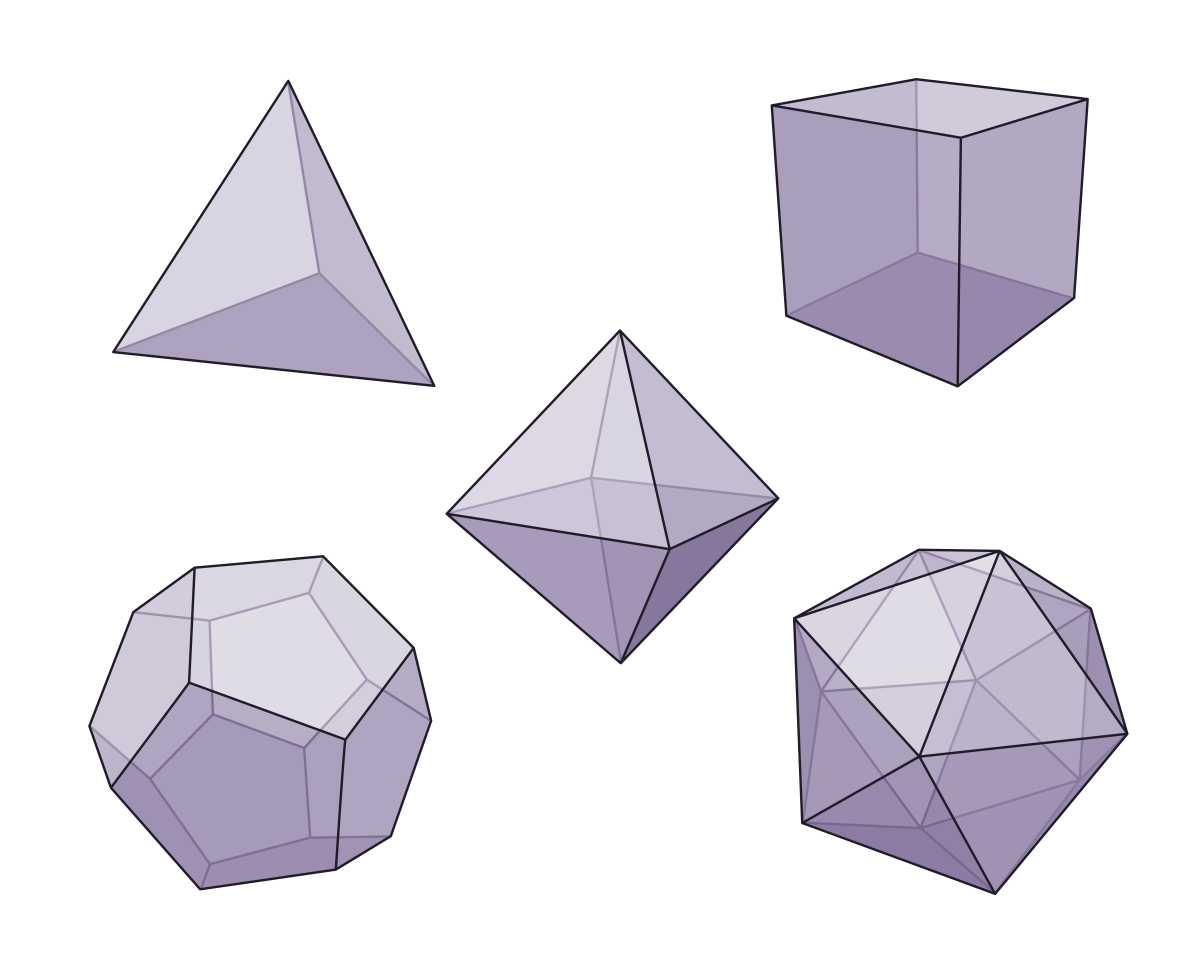
\includegraphics[width=0.9\linewidth]{figures/platonic_solids.png}
The tetrahedron, cube, octahedron, dodecahedron, and icosahedron are called {\em Platonic solids}.}
%
This somewhat poetic definition of symmetry is given in the eponymous book of the great mathematician Hermann \citet{weyl2015symmetry}, his {\em Schwanengesang} on the eve of retirement from the Institute for Advanced Study in Princeton. 
%
Weyl traces the special place symmetry has occupied in science and art to the ancient times, from Sumerian symmetric designs to the Pythagoreans who believed the circle to be perfect due to its rotational symmetry. 
%
Plato considered the five regular polyhedra bearing his name today  so fundamental that they must be the basic building blocks shaping the material world. 
%
Yet, though Plato is credited with coining the term \textgreek{summetr'ia}, which literally translates as `same measure', he used it only vaguely to convey the beauty of proportion in art and harmony in music. 
%
It was the astronomer and mathematician Johannes Kepler to attempt the first rigorous analysis of the symmetric shape of water crystals. In his treatise (`On the Six-Cornered Snowflake'),\marginnote{
%\includegraphics[width=0.9\linewidth]{figures/de_nive.png}
Fully titled 
{\em Strena, Seu De Nive Sexangula} ('New Year's gift, or on the Six-Cornered Snowflake') was, as suggested by the title, a small booklet sent by Kepler in 1611 as a Christmas gift to his patron and friend Johannes Matthäus Wackher von Wackenfels. } he attributed the six-fold dihedral structure of snowflakes to hexagonal packing of particles -- an idea that though preceded the clear understanding of how matter is formed, still holds today as the basis of crystallography \citep{ball2011retrospect}. 




%D'Arcy Thompson {\em On Growth and Form} appeals to the notions of symmetry to explain the structure of biological life forms. 

\paragraph{Symmetry in Mathematics and Physics}
In modern mathematics, symmetry is almost univocally expressed in the language of group theory. %
The origins of this theory are usually attributed to {\'E}variste Galois, who coined the term and used it to study solvability of polynomial equations in the 1830s. 
%
Two other names associated with group theory are those of Sophus Lie and Felix Klein, who met and worked fruitfully together for a period of time \citep{tobies2019felix}. The former would develop the theory of continuous symmetries that today bears his name; the latter proclaimed group theory to be the organising principle of geometry in his Erlangen Program, which we mentioned in the beginning of this text. Riemannian geometry was explicitly excluded from Klein's unified geometric picture, and it took another fifty years before it was integrated, largely thanks to the work of {\'E}lie Cartan in the 1920s.   

%unified multiple geometries. 

%Physics:  


Emmy Noether, Klein's colleague in G\"ottingen, proved that every differentiable symmetry of the action of a physical system has a corresponding conservation law \citep{variationsprobleme1918nachr}. In physics, it was a stunning result: beforehand, meticulous experimental observation was required to discover fundamental laws such as the conservation of energy, and even then, it was an empirical result not coming from anywhere. Noether’s Theorem --- ``a guiding star to 20th and 21st century physics'', in the words of the Nobel laureate Frank Wilczek --- showed that the conservation of energy emerges from the translational symmetry of time, a rather intuitive idea that the results of an experiment should not depend on whether it is conducted today or tomorrow. 

%That theorem has been a guiding star to 20th and 21st century physics,” says theoretical physicist Frank Wilczek


%[FROM WIKI]
The symmetry\marginnote{Weyl first conjectured (incorrectly) in 1919 that invariance under the change of scale or ``gauge'' was a local symmetry of electromagnetism. The term {\em gauge}, or {\em Eich} in German, was chosen by analogy to the various track gauges of railroads. %Although Weyl's choice of the gauge was initially incorrect, the name ``gauge'' stuck to the approach, and 
After the development of quantum mechanics, \cite{weyl1929elektron} modified the gauge choice by replacing the scale factor with a change of wave phase. See \cite{straumann1996early}.
}  associated with charge conservation is the global {\em gauge invariance} of the electromagnetic field, first appearing in Maxwell's formulation of electrodynamics  \citep{maxwell1865viii};  %This symmetry is related to the fact that the electric and magnetic fields are not changed by different choices of the value representing the zero point of electrostatic potential; 
however, its importance initially remained unnoticed. % in the earliest formulations. 
%
%Similarly unnoticed was Hilbert's derivation of Einstein's equations of general relativity by postulating a symmetry under any change of coordinates. 
The same Hermann Weyl 
who wrote so dithyrambically about symmetry %at the end of his academic career 
is the one who first introduced the concept of gauge invariance in physics in the early 20th century, emphasizing its role as a %symmetry 
principle from which electromagnetism can be {\em derived}. 
%
It took several decades until this fundamental principle — in its generalised form 
%to non-Abelian gauge groups 
developed by \cite{yang1954conservation} — 
proved successful in providing a unified framework to describe the quantum-mechanical behavior of electromagnetism and the weak and strong forces, finally culminating in the Standard Model that captures all the fundamental forces of nature but gravity. 
%
We can thus join another Nobel-winning physicist, Philip \cite{anderson1972more}, in concluding that ``it is only slightly overstating the case to say that physics is the study of symmetry.'' 
%More is Different

% N. Strauman, Early History of Gauge Theories and Weak Interactions




%\michael{[from Taco's thesis]

\paragraph{Early Use of Symmetry in Machine Learning}
In machine learning and its applications to pattern recognition and computer vision, the importance of symmetry has long been recognised. 
%
Early work on designing equivariant feature detectors for pattern recognition was done by \citet{amari1978feature},\marginnote{Shun'ichi Amari is credited as the creator of the field of {\em information geometry} that applies Riemannian geometry models to probability. The main object studied by information geometry is a {\em statistical manifold}, where each point corresponds to a probability distribution. } \citet{kanatani2012group}, and \citet{lenz1990group}. 
%
In the 
neural networks literature, the famous Group Invariance Theorem for Perceptrons
by \citet{minsky2017perceptrons} puts fundamental limitations on the capabilities
of (single-layer) perceptrons to learn invariants. This was one of the primary motivations for studying multi-layer architectures \citep{sejnowski1986learning,shawe1989building,shawe1993symmetries}, which ultimately led to deep learning. 

In the neural network community, {\em Neocognitron} \citep{fukushima1982neocognitron} is credited as the first  implementation of shift invariance in a neural network for ``pattern recognition unaffected by shift in position''. 
%maybe without explicitly realizing this fact. In his influential paper (Fukushima 1980) he laments of the response of perceptrons being ``severely affected by the shift in position and by the distortion in shape of the input patterns'' and concludes that ``their ability for pattern recognition was not so high.'' 
%
His solution came in the form of hierarchical neural network with local connectivity, drawing inspiration from the receptive fields discovered in the visual cortex by the neuroscientists David Hubel and Torsten Wiesel two decades earlier \citep{hubel1959receptive}. \marginnote{This classical work was recognised by the Nobel Prize in Medicine in 1981, which Hubel and Wiesel shared with Roger Sperry. }
%
These ideas culminated in Convolutional Neural Networks in the seminal work of Yann LeCun and co-authors \citep{lecun1998gradient}. 
%
The first work to take a representation-theoretical view on invariant and equivariant neural networks was performed by \citet{wood1996representation}, unfortunately rarely cited. 
%
More recent incarnations of these ideas include the works of \citet{makadia2007correspondence,esteves2020spin}
and one of the authors of this text \citep{cohen2016group}.










%Convolutional neural networks: 



%Shawe-Taylor group equivariance
\paragraph{Graph Neural Networks}
%As to Graph Neural Networks, 
It is difficult to pinpoint exactly when the concept of Graph Neural Networks began to emerge---partly due to the fact that most of the early work  did not place graphs as a first-class citizen, partly since GNNs became practical only in the late 2010s, and partly because this field emerged from the confluence of several research areas. That being said, early forms of graph neural networks can be traced back at least to the 1990s, with examples including Alessandro Sperduti's Labeling RAAM \citep{sperduti1994encoding}, the ``backpropagation through structure'' of %K\"{u}chler and Goller 
\cite{goller1996learning}, and adaptive processing of data structures %by Alessandro Sperduti, Antonina Starita and Paolo Frasconi 
\citep{sperduti1997supervised,frasconi1998general}. While these works were primarily concerned with operating over ``structures'' (often trees or directed acyclic graphs), many of the invariances preserved in their architectures are reminiscent of the GNNs more commonly in use today. 



The first proper treatment of the processing of generic graph structures (and the coining of the term \emph{``graph neural network''}) happened after the turn of the 21st century.\marginnote{Concurrently, Alessio Micheli had proposed the \emph{neural network for graphs} (NN4G) model, which focused on a \emph{feedforward} rather than recurrent paradigm \citep{micheli2009neural}.} Within the Artificial Intelligence lab at the Universit\`{a} degli Studi di Siena (Italy), papers led by Marco Gori and Franco Scarselli have proposed the first ``GNN'' \citep{gori2005new,scarselli2008graph}. They relied on recurrent mechanisms, required the neural network parameters to specify \emph{contraction mappings}, and thus computing node representations by searching for a fixed point---this in itself necessitated a special form of backpropagation \citep{almeida1990learning,pineda1988generalization} and did not depend on node features at all. All of the above issues were rectified by the Gated GNN (GGNN) model of \cite{li2015gated}. GGNNs brought many benefits of modern RNNs, such as gating mechanisms \citep{cho2014learning} and backpropagation through time, to the GNN model, and remain popular today.


\paragraph{Computational chemistry}
It is also very important to note an independent and concurrent line of development for GNNs: one that was entirely driven by the needs of computational chemistry, where 
 molecules are most naturally expressed as graphs of atoms (nodes) connected by chemical bonds (edges). 
 %
 This invited computational techniques for molecular property prediction that operate directly over such a graph structure, which had become present in machine learning in the 1990s: this includes the ChemNet model of %Dmitri Kireev 
 \cite{kireev1995chemnet} and the work of %Igor Baskin 
 \cite{baskin1997neural}. Strikingly, the ``molecular graph networks'' of \cite{merkwirth2005automatic} explicitly proposed many of the elements commonly found in contemporary GNNs---such as edge type-conditioned weights or global pooling---as early as 2005. The chemical motivation continued to drive GNN development into the 2010s, with two significant GNN advancements centered around improving molecular fingerprinting \citep{duvenaud2015convolutional} and predicting quantum-chemical properties \citep{gilmer2017neural} from small molecules. 
 %
 At the time of writing this text, molecular property prediction is one of the most successful applications of GNNs, with impactful results in virtual screening of new antibiotic drugs \citep{stokes2020deep}.
 %that has led to the discovery of a novel potent antibiotic drug Halicin \citep{stokes2020deep}.



\paragraph{Node embeddings} Some of the earliest success stories of deep learning on graphs involve learning representations of nodes in an unsupervised fashion, based on the graph structure. Given their structural inspiration, this direction also provides one of the most direct links between graph representation learning and network science communities. The key early approaches in this space relied on \emph{random walk}-based embeddings: learning node representations in a way that brings them closer together if the nodes co-occur in a short random walk. Representative methods in this space include DeepWalk \citep{perozzi2014deepwalk}, node2vec \citep{grover2016node2vec} and LINE \citep{tang2015line}, which are all purely self-supervised. Planetoid \citep{yang2016revisiting} was the first in this space to incorporate supervision label information, when it is available.

Unifying random walk objectives with GNN encoders\marginnote{Recently, a theoretical framework was developed by \citet{srinivasan2019equivalence} in which the equivalence of structural and positional representations was demonstrated. Additionally, \citet{qiu2018network} have demonstrated that all random-walk based embedding techniques are equivalent to an appropriately-posed matrix factorisation task.} was attempted on several occasions, with representative approaches including Variational Graph Autoencoder (VGAE,  \cite{kipf2016variational}), embedding propagation \citep{garcia2017learning}, and unsupervised variants of GraphSAGE \citep{hamilton2017inductive}. However, this was met with mixed results, and it was shortly discovered that pushing neighbouring node representations together is already a key part of GNNs' inductive bias. Indeed, it was shown that an \emph{untrained} GNN was already showing performance that is competitive with DeepWalk, in settings where node features are available \citep{velickovic2019deep,wu2019simplifying}. This launched a direction that moves away from combining random walk objectives with GNNs and shifting towards \emph{contrastive} approaches inspired by mutual information maximisation and aligning to successful methods in the image domain. Prominent examples of this direction include Deep Graph Informax (DGI,  \cite{velickovic2019deep}), GRACE \citep{zhu2020deep}, BERT-like objectives \citep{hu2020strategies} and BGRL \citep{thakoor2021bootstrapped}.

\paragraph{Probabilistic graphical models} 
Graph neural networks have also, concurrently, resurged through embedding the computations of \emph{probabilistic graphical models} (PGMs, \cite{wainwright2008graphical}).
%
PGMs are a powerful tool for processing graphical data, and their utility arises from their probabilistic perspective on the graph's edges: namely, the nodes are treated as \emph{random variables}, while the graph structure encodes \emph{conditional independence} assumptions, allowing for significantly simplifying the calculation and sampling from the joint distribution. Indeed, many algorithms for (exactly or approximately) supporting learning and inference on PGMs rely on forms of passing messages over their edges \citep{pearl2014probabilistic}, with examples including variational mean-field inference and loopy belief propagation \citep{yedidia2001bethe,murphy2013loopy}.

This connection between PGMs and message passing was subsequently developed into GNN architectures, with early theoretical links established by the authors of structure2vec \citep{dai2016discriminative}. Namely, by posing a graph representation learning setting as a Markov random field (of nodes corresponding to input features and latent representations), the authors directly align the computation of both mean-field inference and loopy belief propagation to a model not unlike the GNNs commonly in use today. 

The key ``trick'' which allowed for relating the latent representations of a GNN to probability distributions maintained by a PGM was the usage of \emph{Hilbert-space embeddings} of distributions \citep{smola2007hilbert}. Given $\phi$, an appropriately chosen embedding function for features $\vec{x}$, it is possible to embed their probability distribution $p(\vec{x})$ as the \emph{expected} embedding $\mathbb{E}_{\vec{x}\sim p(\vec{x})}\phi(\vec{x})$. Such a correspondence allows us to perform GNN-like computations, knowing that the representations computed by the GNN will always correspond to an embedding of \emph{some} probability distribution over the node features.

The structure2vec model itself is, ultimately, a GNN architecture which easily sits within our framework, but its setup has inspired a series of GNN architectures which more directly incorporate computations found in PGMs. Emerging examples have successfully combined GNNs with conditional random fields \citep{gao2019conditional,spalevic2020hierachial}, relational Markov networks \citep{qu2019gmnn} and Markov logic networks \citep{zhang2020efficient}.

\paragraph{The Weisfeiler-Lehman formalism} The resurgence of graph neural networks was followed closely by a drive to understand their fundamental limitations, especially in terms of expressive power. While it was becoming evident that GNNs are a strong modelling tool of graph-structured data, it was also clear that they wouldn't be able to solve \emph{any} task specified on a graph perfectly.\marginnote{Due to their permutation invariance, GNNs will attach identical representations to two isomorphic graphs, so this case is trivially solved.} A canonical illustrative example of this is deciding \emph{graph isomorphism}: is our GNN able to attach different representations to two given non-isomorphic graphs? This is a useful framework for two reasons. If the GNN is unable to do this, then it will be hopeless on any task requiring the discrimination of these two graphs. Further, it is currently not known if deciding graph isomorphism is in \textsc{P}\marginnote{The best currently known algorithm for deciding graph isomorphism is due to \citet{babai1983canonical}, though a recent (not fully reviewed) proposal by \citet{babai2016graph} implies a quasi-polynomial time solution.}, the complexity class in which all GNN computations typically reside.

The key framework which binds GNNs to graph isomorphism is the \emph{Weisfeiler-Lehman} (WL) graph isomorphism test \citep{weisfeiler1968reduction}. This test generates a graph representation by iteratively passing node features along the edges of the graph, then \emph{randomly hashing} their sums across neighbourhoods. Connections to \emph{randomly-initialised} convolutional GNNs are apparent, and have been observed early on: for example, within the GCN model of \citet{kipf2016semi}. Aside from this connection, the WL iteration was previously introduced in the domain of \emph{graph kernels} by \citet{shervashidze2011weisfeiler}, and it still presents a strong baseline for unsupervised learning of whole-graph representations.

While\marginnote{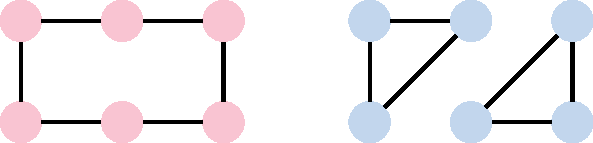
\includegraphics[width=\linewidth]{figures/tikz_WL.pdf} One simple example: the WL test cannot distinguish a \emph{6-cycle} from \emph{two triangles}.} the WL test is conceptually simple, and there are many simple examples of non-isomorphic graphs it cannot distinguish, its expressive power is ultimately strongly tied to GNNs. Analyses by \citet{morris2019weisfeiler} and \citet{xu2018powerful} have both reached a striking conclusion: \emph{any} GNN conforming to one of the three flavours we outlined in Section \ref{sec:gnn-intro} cannot be more powerful than the WL test!

In order to exactly reach this level of representational power, certain constraints must exist on the GNN update rule. \citet{xu2018powerful} have shown that, in the discrete-feature domain, the aggregation function the GNN uses must be \emph{injective}, with \emph{summation} being a key representative\marginnote{Popular aggregators such as maximisation and averaging fall short in this regard, because they would not be able to distinguish e.g. the neighbour multisets $\ldblbrace \vec{a}, \vec{b}\rdblbrace$ and $\ldblbrace \vec{a}, \vec{a}, \vec{b}, \vec{b}\rdblbrace$.}. Based on the outcome of their analysis, \citet{xu2018powerful} propose the Graph Isomorphism Network (GIN), which is a simple but powerful example of a maximally-expressive GNN under this framework. It is also expressible under the convolutional GNN flavour we propose.

Lastly, it is worth noting that these findings do not generalise to \emph{continuous} node feature spaces. In fact, using the Borsuk-Ulam theorem \citep{borsuk1933drei}, \citet{corso2020principal} have demonstrated that, assuming real-valued node features, obtaining injective aggregation functions requires \emph{multiple} aggregators (specifically, equal to the \emph{degree} of the receiver node)\marginnote{One example of such aggregators are the \emph{moments} of the multiset of neighbours.}. Their findings have driven the Principal Neighbourhood Aggregation (PNA) architecture, which proposes a multiple-aggregator GNN that is empirically powerful and stable.

\paragraph{Higher-order methods} % and Topological Data Analysis}

The findings of the previous paragraphs do not contradict the practical utility of GNNs. Indeed, in many real-world applications the input features are sufficiently \emph{rich} to support useful discriminative computations over the graph structure, despite of the above limitations\marginnote{Which, in contrast, almost always consider \emph{featureless} or \emph{categorically-featured} graphs.}. 

However, one key corollary is that GNNs are relatively quite weak at detecting some rudimentary \emph{structures} within a graph. Guided by the specific limitations or failure cases of the WL test, several works have provided \emph{stronger} variants of GNNs that are \emph{provably} more powerful than the WL test, and hence likely to be useful on tasks that require such structural detection\marginnote{One prominent example is computational chemistry, wherein a molecule's chemical function can be strongly influenced by the presence of aromatic \emph{rings} in its molecular graph.}.

Perhaps the most direct place to hunt for more expressive GNNs is the WL test itself. Indeed, the strength of the original WL test can be enhanced by considering a \emph{hierarchy} of WL tests, such that $k$-WL tests attach representations to $k$\emph{-tuples} of nodes \citep{morris2017glocalized}. The $k$-WL test has been directly translated into a \emph{higher-order} $k$-GNN architecture by \citet{morris2019weisfeiler},\marginnote{There have been efforts, such as the $\delta$-$k$-LGNN \citep{morris2020weisfeiler}, to sparsify the computation of the $k$-GNN.} which is provably more powerful than the GNN flavours we considered before. However, its requirement to maintain tuple representations implies that, in practice, it is hard to scale beyond $k=3$.

Concurrently, \citet{maron2018invariant,maron2019provably} have studied the characterisation of invariant and equivariant graph networks over $k$-tuples of nodes. Besides demonstrating the surprising result of \emph{any} invariant or equivariant graph network being expressible as a linear combination of a finite number of generators---the amount of which only depends on $k$---the authors showed that the expressive power of such layers is equivalent to the $k$-WL test, and proposed an empirically scalable variant which is provably 3-WL powerful.

Besides generalising the domain over which representations are computed, significant effort had also went into analysing specific failure cases of 1-WL and augmenting GNN \emph{inputs} to help them distinguish such cases. One common example is attaching \emph{identifying features} to the nodes, which can help detecting structure\marginnote{For example, if a node sees its own identifier $k$ hops away, it is a direct  indicator that it is within a $k$-cycle.}. Proposals to do this include \emph{one-hot} representations \citep{murphy2019relational}, as well as purely \emph{random} features \citep{sato2020random}.

More broadly, there have been many efforts to incorporate \emph{structural} information within the message passing process, either by modulating the message function or the graph that the computations are carried over\marginnote{In the computational chemistry domain, it is often assumed that molecular function is driven by substructures (the \emph{functional groups}), which have directly inspired the modelling of molecules at a \emph{motif} level. For references, consider \cite{jin2018junction,jin2020hierarchical,fey2020hierarchical}.}. Several interesting lines of work here involve sampling \emph{anchor node sets} \citep{you2019position}, aggregating based on \emph{Laplacian eigenvectors} \citep{stachenfeld2020graph,beaini2020directional,dwivedi2020generalization}, or performing \emph{topological data analysis}, either for positional embeddings \citep{bouritsas2020improving} or driving message passing \citep{bodnar2021weisfeiler}.

 
% Lastly, it is important to note that one of the most popularised and impactful applications of graph representation learning at the time of writing this book exactly corresponds to using GNNs to accurately screen potential drugs, leading to discovery of a novel potent antibiotic, Halicin \citep{stokes2020deep}. 

%\michael{
\paragraph{Signal processing and Harmonic analysis}
Since the early successes of Convolutional Neural Networks, researchers have resorted to tools from harmonic analysis, image processing, and computational neuroscience trying to provide a theoretical framework that explains their efficiency. 
$M$-theory is a framework inspired by the visual cortex, pioneered by Tomaso Poggio and collaborators \citep{riesenhuber1999hierarchical, serre2007feedforward}, based on the notion of templates that can be manipulated under certain symmetry groups. Another notable model arising from computational neuroscience were {\em steerable pyramids}, a form of multiscale wavelet decompositions  with favorable properties against certain input transformations, developed by \cite{simoncelli1995steerable}. They were a central element in early generative models for textures \citep{portilla2000parametric}, which were subsequently improved by replacing steerable wavelet features with deep CNN features \cite{gatys2015texture}. 
Finally, Scattering transforms, introduced by St{\'e}phane \cite{mallat2012group} and developed by \cite{bruna2013invariant}, provided a framework to understand CNNs by replacing trainable filters with multiscale wavelet decompositions, also showcasing the deformation stability and the role of depth in the architecture.  


% Wavelets Mallat

% Multiscale analysis

% Simoncelli

% Poggio
%}


%[spectral]

\paragraph{Signal Processing on Graph and Meshes}
Another important class of graph neural networks, often referred to as {\em spectral}, has emerged from the work of one of the authors of this text \citep{bruna2013spectral}, using the notion of the \emph{Graph Fourier transform}.  
%
The roots of this construction are in the signal processing and computational harmonic analysis communities, where dealing with non-Euclidean signals has become prominent in the late 2000s and early 2010s. Influential papers from the groups of Pierre Vandergheynst \citep{shuman2013emerging} and Jos{\'e} Moura \citep{sandryhaila2013discrete} popularised the notion of ``Graph Signal Processing'' (GSP) and the generalisation of Fourier transforms based on the eigenvectors of graph adjacency and Laplacian matrices. 
%
The graph convolutional neural networks relying on spectral filters by  \citet{defferrard2016convolutional} and \cite{kipf2016semi} are among the most cited in the field and can likely be credited) as ones  reigniting the interest in machine learning on graphs in recent years.  


It is worth noting that, in the field of computer graphics and geometry processing, non-Euclidean harmonic analysis predates Graph Signal Processing by at least a decade. We can trace spectral filters on manifolds and meshes to the works of \cite{taubin1996optimal}. These methods became mainstream in the 2000s following the influential papers of %Zachi Karni and Craig Gotsman 
\cite{karni2000spectral} on spectral geometry compression and of \cite{levy2006laplace} on using the Laplacian eigenvectors as a non-Euclidean Fourier basis. 
%
Spectral methods have been used for a range of applications,\marginnote{Learnable shape descriptors similar to spectral graph CNNs were proposed by Roee Litman and Alex Bronstein (\citeyear{litman2013learning}), the latter being a twin brother of the author of this text. } most prominent of which is the construction of shape descriptors \citep{sun2009concise} and functional maps \citep{ovsjanikov2012functional}; these methods are still broadly used in computer graphics at the time of writing. 


%\michael{Kova\v{c}evi\'{c}}




\paragraph{Computer Graphics and Geometry Processing}
%\michael{Metric models, isometry-invariance, symmetry}
Models for shape analysis based on intrinsic metric invariants were introduced by various authors in the field of computer graphics and geometry processing \citep{elad2003bending,memoli2005theoretical,bronstein2006generalized}, and are discussed in depth by one of the authors in his earlier book \citep{bronstein2008numerical}. The notions of intrinsic symmetries were also explored in the same field  \cite{raviv2007symmetries,ovsjanikov2008global}. 
%
The first architecture for deep learning on meshes, Geodesic CNNs, was developed in the team of one of the authors of the text \citep{masci2015geodesic}. This model used local filters with shared weights, applied to geodesic radial patches. It was a particular setting of gauge-equivariant CNNs developed later by another author of the text \citep{cohen2019gauge}. 
%
A generalisation of Geodesic CNNs with learnable aggregation operations, MoNet, proposed by Federico  \cite{monti2017geometric} from the same team, used an attention-like mechanism over the local structural features of the mesh, that was demonstrated to work on general graphs as well. 
%
The graph attention network (GAT), which technically speaking can be considered a particular instance of MoNet, was introduced by another author of this text \citep{velickovic2018graph}. GATs generalise MoNet's attention mechanism to also incorporate node feature information, breaking away from the purely structure-derived relevance of prior work. It is one of the most popular GNN architectures currently in use.


In the context of computer graphics, it is also worthwhile to mention that the idea of learning on sets \citep{zaheer2017deep} was concurrently developed in the group of Leo Guibas at Stanford under the name PointNet \citep{qi2017pointnet} for the analysis of 3D point clouds. This architecture has lead to multiple follow-up works, including one by an author of this text called Dynamic Graph CNN (DGCNN, \cite{wang2019dynamic}). DGCNN used a nearest-neighbour graph to capture the local structure of the point cloud to allow exchange of information across the nodes; the key characteristic of this architecture was that the graph was constructed on-the-fly and updated between the layers of the neural network in relation to the downstream task. 
%
This latter property made DGCNN one of the first incarnations of `latent graph learning', which in its turn has had significant follow up. Extensions to DGCNN's $k$-nearest neighbour graph proposal include more explicit control over these graphs' edges, either through bilevel optimisation \citep{franceschi2019learning}, reinforcement learning \citep{kazi2020differentiable} or direct supervision \citep{velivckovic2020pointer}. Independently, a variational direction (which probabilistically samples edges from a computed \emph{posterior} distribution) has emerged through the NRI model \citep{kipf2018neural}. While it still relies on quadratic computation in the number of nodes, it allows for explicitly encoding uncertainty about the chosen edges.
%\michael{Mention algorithmic reasoning and Cranmer's work on symbolic equations?}

Another very popular direction in learning on graphs without a provided graph relies on performing GNN-style computations over a \emph{complete} graph, letting the network infer its own way to exploit the connectivity. The need for this arisen particularly in natural language processing, where various words in a sentence interact in highly nontrivial and non-sequential ways. Operating over a complete graph of words brought about the first incarnation of the Transformer model \citep{vaswani2017attention}, which de-throned both recurrent and convolutional models as state-of-the-art in neural machine translation, and kicked off an avalanche of related work, transcending the boundaries between NLP and other fields. Fully-connected GNN computation has also concurrently emerged on simulation \citep{battaglia2016interaction}, reasoning \citep{santoro2017simple}, and multi-agent \citep{hoshen2017vain} applications, and still represents a popular choice when the number of nodes is reasonably small.
%
%Most recent works 

%manifold learning 

%Rotation-equivariant CNNs

\paragraph{Algorithmic reasoning} 
For most of the discussion we posed in this section, we have given examples of \emph{spatially} induced geometries, which in turn shape the underlying domain, and its invariances and symmetries. However, plentiful examples of invariances and symmetries also arise in a \emph{computational} setting. One critical difference to many common settings of Geometric Deep Learning is that links no longer need to encode for any kind of similarity, proximity, or types of relations---they merely specify the ``recipe'' for the dataflow between data points they connect.

Instead, the computations of the neural network mimic the reasoning process of an \emph{algorithm} \citep{cormen2009introduction}, with additional invariances induced by the algorithm's control flow and intermediate results\marginnote{For example, one invariant of the Bellman-Ford pathfinding algorithm \citep{bellman1958routing} is that, after $k$ steps, it will always compute the shortest paths to the source node that use no more than $k$ edges.}. In the space of algorithms the assumed input invariants are often referred to as \emph{preconditions}, while the invariants preserved by the algorithm are known as \emph{postconditions}.

Eponymously, the research direction of \emph{algorithmic reasoning} \citep[Section 3.3.]{cappart2021combinatorial} seeks to produce neural network architectures that appropriately preserve algorithmic invariants. The area has investigated the construction of general-purpose neural computers, e.g., the \emph{neural Turing machine} \citep{graves2014neural} and the \emph{differentiable neural computer} \citep{graves2016hybrid}. While such architectures have all the hallmarks of general computation, they introduced several components at once, making them often challenging to optimise, and in practice, they are almost always outperformed by simple relational reasoners, such as the ones proposed by \citet{santoro2017simple,santoro2018relational}. 

As modelling complex postconditions is challenging, plentiful work on inductive biases for learning to execute \citep{zaremba2014learning} has focused on primitive algorithms (e.g. simple arithmetic). Prominent examples in this space include the \emph{neural GPU} \citep{kaiser2015neural}, \emph{neural RAM} \citep{kurach2015neural}, \emph{neural programmer-interpreters} \citep{reed2015neural}, \emph{neural arithmetic-logic units} \citep{trask2018neural,madsen2020neural} and \emph{neural execution engines} \citep{yan2020neural}.

Emulating combinatorial algorithms of \emph{superlinear} complexity was made possible with the rapid development of GNN architectures. The \emph{algorithmic alignment} framework pioneered by \citet{xu2019can} demonstrated, theoretically,  that GNNs \emph{align} with dynamic programming \citep{bellman1966dynamic}, which is a language in which most algorithms can be expressed. It was concurrently empirically shown, by one of the authors of this text, that it is possible to design and train GNNs that align with algorithmic invariants in practice \citep{velivckovic2019neural}. Onwards, alignment was achieved with \emph{iterative algorithms} \citep{tang2020towards}, \emph{linearithmic algorithms} \citep{freivalds2019neural}, \emph{data structures} \citep{velivckovic2020pointer} and \emph{persistent memory} \citep{strathmann2021persistent}. Such models have also seen practical use in \emph{implicit planners} \citep{deac2020xlvin}, breaking into the space of \emph{reinforcement learning} algorithms.

Concurrently, significant progress has been made on using GNNs for \emph{physics simulations} \citep{sanchez2020learning,pfaff2020learning}. This direction yielded much of the same recommendations for the design of generalising GNNs. Such a correspondence is to be expected: given that algorithms can be phrased as discrete-time simulations, and simulations are typically implemented as step-wise algorithms, both directions will need to preserve similar kinds of invariants.

Tightly bound with the study of algorithmic reasoning are measures of \emph{extrapolation}. This is a notorious pain-point for neural networks, given that most of their success stories are obtained when  generalising \emph{in-distribution}; i.e. when the patterns found in the training data properly anticipate the ones found in the test data. However, algorithmic invariants must be preserved irrespective of, e.g., the size or generative distribution of the input, meaning that the training set will likely not cover any possible scenario encountered in practice. \citet{xu2020neural} have proposed a geometric argument for what is required of an extrapolating GNN backed by rectifier activations: its components and featurisation would need to be designed so as to make its constituent modules (e.g. message function) learn only \emph{linear} target functions. \citet{bevilacqua2021size} propose observing extrapolation under the lens of \emph{causal reasoning}, yielding \emph{environment-invariant} representations of graphs.

\paragraph{Geometric Deep Learning}
Our final historical remarks regard the very name of this text.
%
The term `Geometric Deep Learning' was first introduced by one of the authors of this text in his ERC grant in 2015 and popularised in the eponymous IEEE Signal Processing Magazine paper \citep{bronstein2017geometric}. This paper proclaimed, albeit ``with some caution'', the signs of ``a new field being born.'' Given the recent popularity of graph neural networks, the increasing use of ideas of invariance and equivariance in a broad range of machine learning applications, and the very fact of us writing this text, it is probably right to consider this prophecy at least partially fulfilled. 
%
The name ``4G: Grids, Graphs, Groups, and Gauges'' was coined by Max Welling for the ELLIS Program on Geometric Deep Learning, co-directed by two authors of the text. Admittedly, the last `G' is somewhat of a stretch, since the underlying structures are manifolds and bundles rather than gauges. 
%
For this text, we added another `G', Geodesics, in reference to metric invariants and intrinsic symmetries of manifolds. 


%{\footnotesize 